\documentclass{../res/univ-projet}

%Import des packages utilisés pour le document
\usepackage[utf8x]{inputenc}
\usepackage[francais]{babel}
\usepackage[T1]{fontenc}

%Redéfinition des marges
\addtolength{\topmargin}{-1cm}
\addtolength{\textheight}{1cm}
\addtolength{\headsep}{0.8cm}
\addtolength{\footskip}{-0.2cm}

%Variables
\logo{../res/logo_univ.png}
\title{Document d'architecture du logiciel}
\author{Matthieu \bsc{Fin}, Guillaume \bsc{Leroy}}
\projet{GPG}
\projdesc{Interface Graphique GPG}
\filiere{M1SSI - Conduite de Projet}
\version{0.1}
\relecteur{}
\signataire{Magali \bsc{Bardet}}
\date{\today}


\histentry{0.1}{23/11/2014}{Version initiale.}

% -- Début du document -- %
\begin{document}

%Page de garde
\maketitle
\newpage
%La table des matières
\tableofcontents
\newpage

\section{Objet}
  \textcolor{blue}{
    TODO : i\\
    Définir les objectifs du document et présenter son contenu en rappelant le
    besoin en quelques phrases. Mettre en exergue les exigences les plus importantes.
  }


\section{Documents applicables et de référence}
  \textcolor{blue}{
    TODO : \\
    Lister \\
    {\begin{itemize}
      \item Les références des documents de spécification.
      \item Les références des documents cités par la suite au titre d'explication ou de 
      justification.
    \end{itemize}}
  }

\section{Terminologie et sigles utilisés}
  \textcolor{blue}{
    TODO : \\
    {\begin{itemize}
      \item Glossaire ou dictionnaire.
      \item Abréviations.
      \item Formalisme utilisé.
      \item Légendes et conventions de représentation.
    \end{itemize}}
  }

\section{Configuration et sigles utilisés}
  \textcolor{blue}{
    TODO : \\
    Décrire les caractéristiques de la plate-forme cible. \\
    {\begin{itemize}
      \item Performances du calculateur.
      \item Périphériques et matériels spécifiques.
      \item système d'exploitation (type et version).
      \item Liste ou tableau des poduits logiciels nécessaires (noms, origines, type et versions).
    \end{itemize}}
  }

\section{Architecture statique}
  \subsection{Structure} % (fold)
    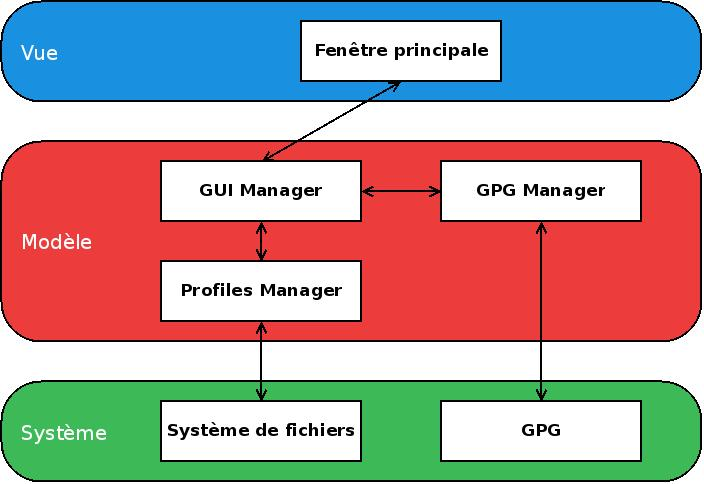
\includegraphics[scale=0.5]{diagramme_archi.jpg}
    %\textcolor{blue}{
    %  TODO : \\
    %  Identifier les principaux constituants du logiciel à développer et présenter la structure statique dans laquelle ils s’intègrent sous la forme d’une « carte de l’architecture » (schéma descriptif faisant apparaître les constituants et leurs interdépendances)
    %}

  % subsection structure (end)
  \subsection{Description du constituant "X"} % (fold)
    \textcolor{blue}{
      TODO : \\
      {\begin{itemize}
        \item Rôle.
        \item Propriétés et attributs de caractérisation.
        \item Services offert (interfaces)
        \item Dépendances avec d'autres constituants (service utilisés,
        composants "sur étagère" utilisés)
        \item Langage de programmation
        \item Procédé de développement (techniques, méthodes et/ou outils)
        \item Taille et complexité.
      \end{itemize}}
    }
  % subsection Description du constituant "X" (end)
  \subsection{Justification techniques} % (fold)
    \textcolor{blue}{
      TODO : \\
      Fournir une rapide justification des choix technique originaux.
    }
  % subsection justification_techniques (end)
\section{Fonctionnement dynamique} % (fold)
\label{sec:fonctionnement_dynamique}

  \textcolor{blue}{
    TODO : \\
    Pour les principaux scénarii identifiés dans la spécification technique de besoin.
    \begin{itemize}
      \item Liste des composants mis en jeu.
      \item Description du processus de mise en oeuvre sous la forme d'une
      séquence d'appels aux services offerts par les différents composants et en faisant
      clairement apparaître
      \begin{itemize}
        \item la logique et le flux des événements traités
        \item les interactions du logiciels avec les acteurs
        \item les interactions entre les composants au travers de leurs interfaces
      \end{itemize}
    \end{itemize}
  }

% section fonctionnement_dynamique (end)
\section{Traçabilité} % (fold)
\label{sec:tra_abilit_}

  \textcolor{blue}{
    TODO : \\
    Récapitulatif des liens de dépendance entre les constituants du logiciel et les exigences de
    la STB (par exemple sous forme de tableau).
  }

% section tra_abilit_ (end)
\end{document}

